% This file demonstrates how to use the IEEEConf LaTeX2e macro package,
% to prepare a manuscript for proceedings on CD of the conference
% FedCSIS
%
\documentclass[a4paper, conference]{IEEEtran}
%\documentclass[a4paper]{IEEEconf}

% This package serves to balance the column lengths on the last page of the document.
% please, insert \balance command in the left column of the last page

\usepackage{balance}

%% to enable \thank command
\IEEEoverridecommandlockouts
%% The usage of the following packages is recommended
%% to insert graphics
%\usepackage[dvips]{graphicx}
% to typeset algorithms
\usepackage{algorithmic}
\usepackage{algorithm}
% to typeset code fragments
\usepackage{listings}
% to make an accent \k be available
\usepackage[OT4,T1]{fontenc}
% provides various features to facilitate writing math formulas and to improve the typographical quality of their output.
\usepackage[cmex10]{amsmath}
\interdisplaylinepenalty=2500
% por urls typesetting and breaking
\usepackage{url}
% for vertical merging table cells
\usepackage{multirow}

% \usepackage{graphicx}
\usepackage{epstopdf}
\usepackage{graphicx}


%\usepackage[T1]{fontenc}
%\usepackage[utf8]{inputenc}
%\usepackage[slovak]{babel}

\usepackage[slovak, english]{babel}

\usepackage{listings}             % Include the listings-package



% define environments for remarks and examples
\newtheorem{remark}{Remark}[section]
\newtheorem{example}[remark]{Example}

%
%
\title{Real-Time Schedule for Mobile Robotics and WSN Aplications}
%
%
\author{

\IEEEauthorblockN{Michal Chovanec *}
\IEEEauthorblockA{{University of \v{Z}}ilina\\
Faculty of Management Science and Informatics,\\
Univerzitn{\'{a}} 8215/1
{\v{Z}}ilina 010 26, \\
michal.chovanec@fri.uniza.sk}
\and

\IEEEauthorblockN{Peter \v{S}araf\'{i}n}
\IEEEauthorblockA{{University of \v{Z}}ilina\\
Faculty of Management Science and Informatics,\\
Univerzitn{\'{a}} 8215/1
{\v{Z}}ilina 010 26, \\
peter.sarafin@fri.uniza.sk}


}

% conference papers do not typically use \thanks and this command
% is locked out in conference mode. If really needed, such as for
% the acknowledgment of grants, issue a \IEEEoverridecommandlockouts
% after \documentclass

% for over three affiliations, or if they all won't fit within the width
% of the page, use this alternative format:
%
%\author{\IEEEauthorblockN{Michael Shell\IEEEauthorrefmark{1},
%Homer Simpson\IEEEauthorrefmark{2},
%James Kirk\IEEEauthorrefmark{3},
%Montgomery Scott\IEEEauthorrefmark{3} and
%Eldon Tyrell\IEEEauthorrefmark{4}}
%\IEEEauthorblockA{\IEEEauthorrefmark{1}School of Electrical and Computer Engineering\\
%Georgia Institute of Technology,
%Atlanta, Georgia 30332--0250\\ Email: see http://www.michaelshell.org/contact.html}
%\IEEEauthorblockA{\IEEEauthorrefmark{2}Twentieth Century Fox, Springfield, USA\\
%Email: homer@thesimpsons.com}
%\IEEEauthorblockA{\IEEEauthorrefmark{3}Starfleet Academy, San Francisco, California 96678-2391\\
%Telephone: (800) 555--1212, Fax: (888) 555--1212}
%\IEEEauthorblockA{\IEEEauthorrefmark{4}Tyrell Inc., 123 Replicant Street, Los Angeles, California 90210--4321}}





\begin{document}
\maketitle              % typeset the title of the contribution

\begin{abstract}
This paper presents real-time scheduler in operating system running on ARM Cortex (M0, M3, M4) usable in small mobile robotics with kernel response around 1ms. Thanks to the strong modularity, advanced sleep modes and event driven programming ability, it can be used for WSN applications too.
\end{abstract}

keywords : operating system, ARM Cortex M, mobile robotics, WSN node, low-power, real-time

\section{Introduction}

\IEEEPARstart{R}{eal-time} scheduler provides added value for embedded software development in the form of strong modularity, reusable code and rapid development \cite{bib:rad}. Many embedded applications work without operating system - usually single purpose tasks or interrupt driven tasks. For more complex applications, operating system can provide better results when some common problems occure \cite{bib:wsn_applications1} \cite{bib:wsn_applications2} :

\begin{itemize}
  \item Multiple sensors (or any inputs) reading
  \item Multiple control loops with different sampling time
  \item Communication (routing, resending)
  \item Power management
  \item System modularity and extension posibilities
  \item GUI running on background of the main process
\end{itemize}
From these, we can consider following operating system requirements:

\begin{itemize}
	\item Multiple parallel threads (often with priority scheduling)
	\item Real-time processing ability
	\item Code size acceptable for microcontroller abilities
	\item Sleep modes support
	\item Multiplatform compilation ability
	\item Modular architecture
\end{itemize}


\section{Sytem architecture}

The operating system runs on a single chip microcontroller. Supported cores are ARM Cortex M0, M0+, M3, M4 and M4F. For testing, TI TivaC TM4C123G \cite{bib:ti_launchpad} (Fig. \ref{fig_ti_launchpad}) with cortex M4F core has been used. This MCU is running on 80MHz and it disposes 256K flash memory and 32K SRAM. Other devices, such as STM32L053, STM32F103, STM32F407, LPC812, MKL02Z32 and MKL25Z4 have also been tested.

All parts are compiled using GNU GCC (using C99 standard) into single binary file, which can be loaded into flash memory \cite{bib:lm4flash}. Recent source files can be downloaded from \cite{bib:suzuha_git}.

Presented operating system consists of these parts:

\begin{itemize}
	\item User application
	\item User libraries
	\item Kernel
	\item OS libraries
	\item Device low level libraries
\end{itemize}

All parts can work independently on each other. Only necessary part is device low level libraries, represented as HAL
(hardware abstraction layer). Operating system is written with microkernel architecture, where kernel only creates and schedules threads. Other functions are implemented as optional libraries.

\renewcommand{\figurename}{Fig.}
\begin{figure}[!t]
\centering
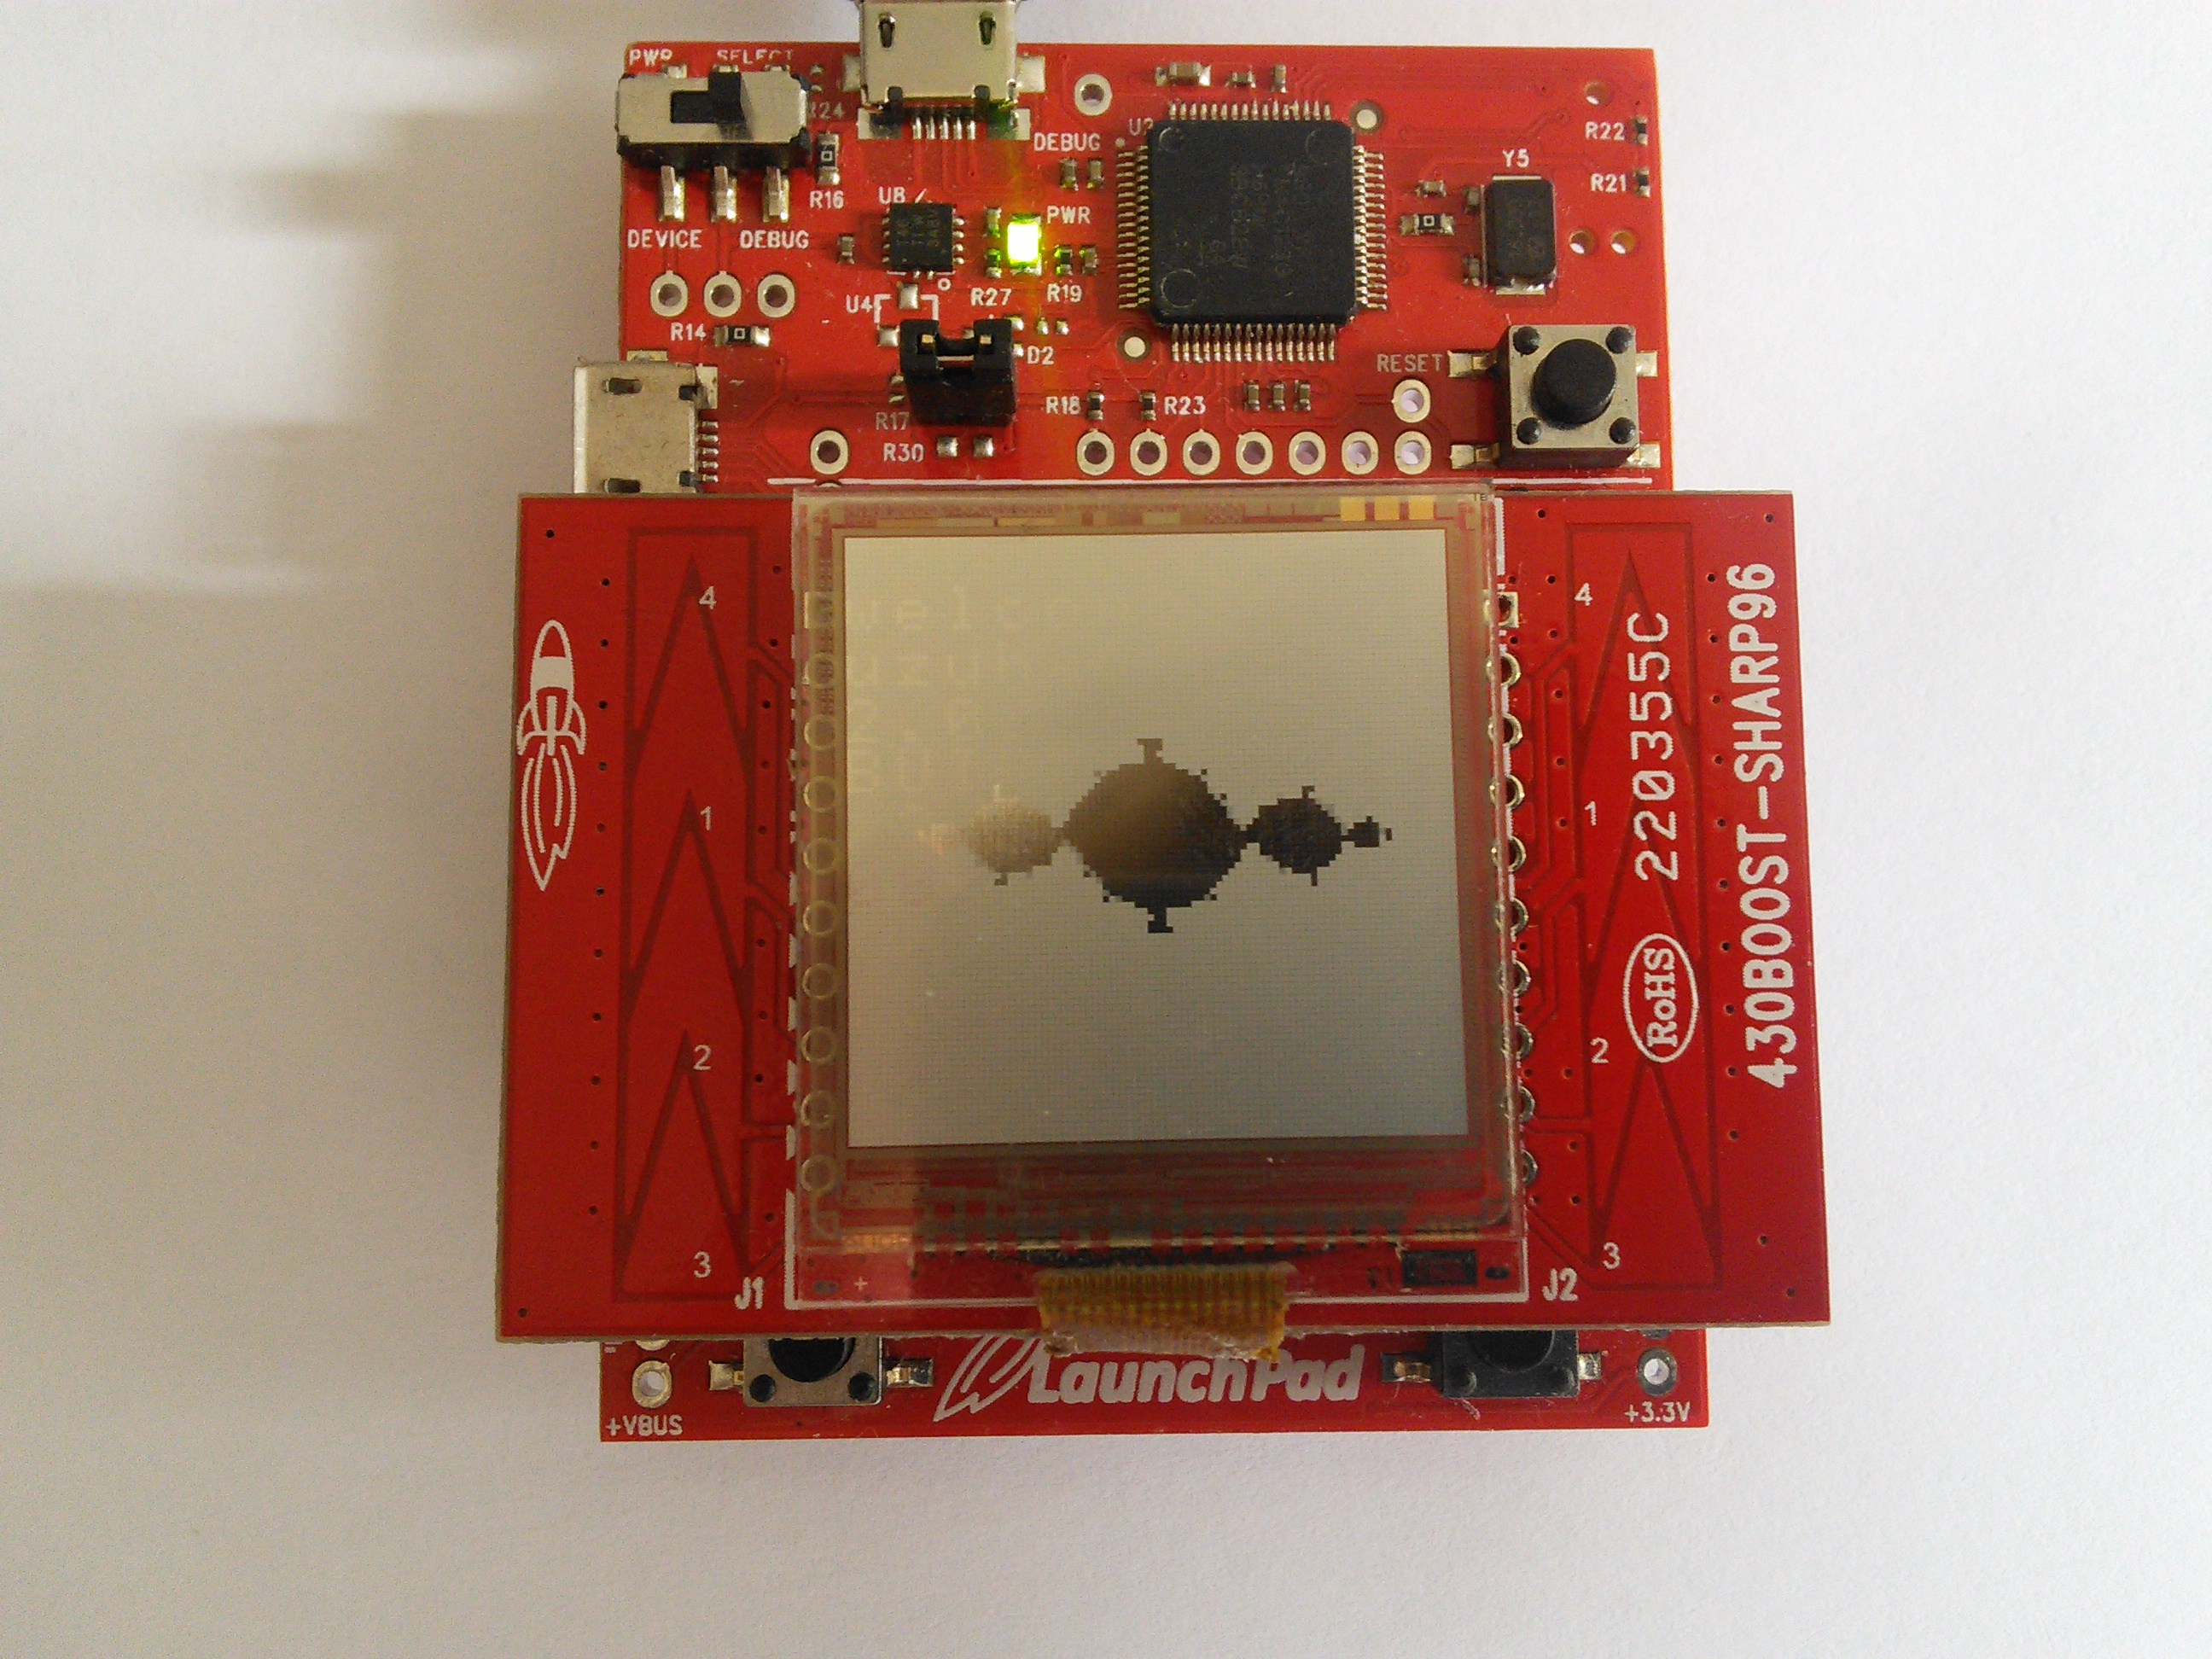
\includegraphics[width=3.2in]{testing_board_01.jpg}
\caption{TI TivaC launchpad testing board}
\label{fig_ti_launchpad}
\end{figure}

In the following text, we briefly describe OS structure. The priority scheduling algorithm compared with common round robin is described in more details.

\subsection{Booting process}

After microcontroller reset, HAL is initialized first, especially clock configuration, GPIO initialization, UART timers and ADC setup.
All parts are initialized only if they are linked in the binary. In other case, initialization of missing parts is skipped.
Absolute minimum requirement for OS running is main clock initialization. For common problems, UART and timers are necessary.

Operating system libraries such as STDIO, software timers, messages subsystem and mutexes are initialized next.
After this, kernel is initialized and user main thread is started.

\subsection{User application and libraries}

Users main loop is discussed in this section. The main function is called $void\ main\_thread()$. This main thread can create other threads, by calling $create\_thread$ function. Following code shows how another thread can be created. When $void\ main\_thread()$ is running, user can initialize it's own libraries, usually sensors, displays or communication module. Boot up and four running threads screenshot is displayed in  the Fig. \ref{fig_os_terminal}.

\noindent\begin{minipage}{.45\textwidth}
\lstset{language=C++}
\begin{lstlisting}[frame=single, caption = Thread creating]
thread_stack_t thread_01_stack
[THREAD_STACK_SIZE];

void thread_01(){
}

void main_thread(){
    create_thread(
        thread_01,
        thread_01_stack,
        sizeof(thread_01_stack),
        PRIORITY_MAX);

    while (1)
    {
    }
}
\end{lstlisting}
\end{minipage}\hfill


\begin{figure}[!t]
\centering
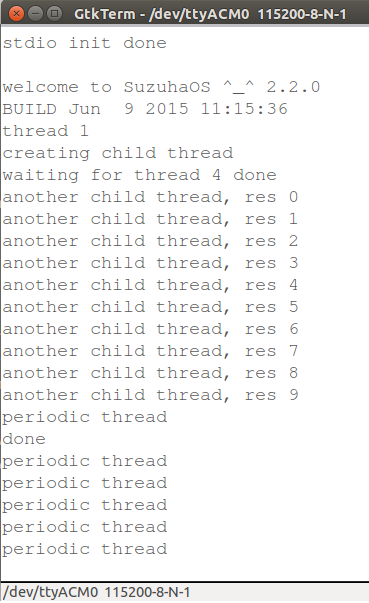
\includegraphics[width=2.5in]{threads.png}
\caption{OS terminal screenshot}
\label{fig_os_terminal}
\end{figure}

\section{Scheduling algorithm}

Main part of OS is the microkernel core. Preemptive multitasking with two options, round robin scheduling or time decrease
priority scheduling is implemented. To compare different schedule algorithms (especially real-time processing), we first need to define error function. Consider set of threads as
\begin{align}
\label{thread}
t_i \in T(p, k, s, d, c) ,
\end{align}
where
$p$ represents thread priority (lower number - higher priority),
$k$ is the counter of thread priority current value,
$s$ stands for thread state (running, waiting, created),
$d$ states thread deadline time (set by user, usually in ms),
$c$ is thread running code (represented as Turing machine).

Let us define thread execution time function as $g(t_i)$ and error function as

\begin{align}
e = \sum_{i=1}^{Tc} |d_i - g(t_i)| ,
\end{align}
where $Tc$ is threads count. This function represents the error, which corresponds with the difference between required deadline time and measured time of running thread.
Using priorities we can define error as

\begin{align}
e = \sum_{i=1}^{Tc} |d_i - g(t_i)|\frac{1}{p_i} ,
\end{align}
where lower $p_i$ means higher priority.

Consider that the faster execution of the thread is not an~issue. This fact means that CPU spends remaining time waiting (executing other threads or sleeping). We can write this as  (\ref{error_equ})  and (\ref{error_eq}).

\begin{align}
\label{error_equ}
	 e_i &=
	  \begin{cases}
	   d_i - g(t_i) & if\ d_i < g(t_i) \\
	   0       & else
	  \end{cases}
\end{align}

\begin{align}
\label{error_eq}
e = \sum_{i=1}^{Tc} |e(t_i)|\frac{1}{p_i}
\end{align}

Threads with higher priority (smaller $p_i$) have bigger influence on the total error. To implement priorities, we define following structure for each thread:
\noindent\begin{minipage}{.45\textwidth}
\lstset{language=C++}
\begin{lstlisting}[frame=single, caption = thread structure]
struct sThread{
    u16 cnt, icnt;
    u32 flag;
    u32 *sp;
};
\end{lstlisting}
\end{minipage}\hfill
where $cnt$ and $icnt$ are counters used for priority scheduling, corresponding with $p$ and $k$ respectively in (\ref{thread}).
When thread is created, $p$ and $k$ are set to $priority$ value and remain constant (variability during execution is also possible, but not tested yet).
Each nonzero $k$ is decremented after each timer interrupt. Thread with smaller $k$ is chosen for the next execution and its $k$ is loaded back to $p$.
Realization in C code is presented on following code listings.
\noindent
\begin{minipage}{.45\textwidth}
\lstset{language=C++}
\begin{lstlisting}[frame=single, caption = priority scheduler]
u32 i, min_i = 0;

/*find thread with minimum cnt*/
for (i = 0; i < THREADS_MAX_COUNT; i++)
{
    if (__thread__[i].cnt <
      __thread__[min_i].cnt)
	min_i=i;

    /*decrement counters*/
    if (__thread__[i].cnt != 0)
	__thread__[i].cnt--;
}

__thread__[min_i].cnt =
	__thread__[min_i].icnt;
__current_thread__ = min_i;
\end{lstlisting}
\end{minipage}
%\hfill
\\
For full function, other common functions like thread creating, waiting or setting into waiting state are implemented.
\noindent\begin{minipage}{.45\textwidth}
\lstset{language=C++}
\begin{lstlisting}[frame=single, caption = kernel functions]

void sched_off();
void sched_on();


void yield();

u32 get_thread_id();

void kernel_init();
void kernel_start();

u32 create_thread(
    void (*thread_ptr)(),
    thread_stack_t *s_ptr,
    u32 stack_size,
    u16 priority);

void kernel_panic();

void set_wait_state();
void wake_up_threads();
void wake_up_threads_int();

void join(u32 thread_id);

\end{lstlisting}
\end{minipage}\hfill



\section{Experimental results}

\begin{figure}[]
\centering
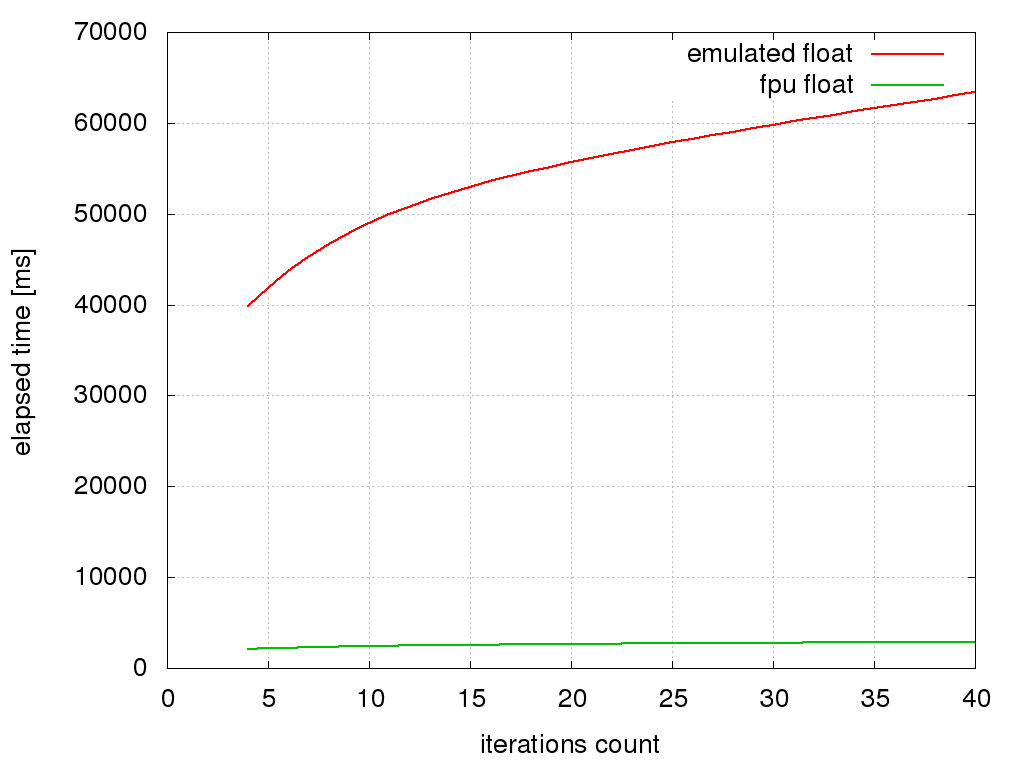
\includegraphics[width=3.4in]{fpu_cpu_performance.png}
\caption{FPU and CPU calculation times}
\label{fig_fpu_cpu}
\end{figure}

For testing OS, few experiments were performed. First one was aimed for the basic multitasking test and comparison of performance using hardware and software emulated float performance.
There were four running threads in this experiment. One thread was calculating Julia set fractal and results were displayed on LCD. Total number of calculating points was set to 96x96.
Quantity of algorithm iterations was changing from interval $\langle 4, 40 \rangle$. Performance result is represented in the Fig.~\ref{fig_fpu_cpu}. In this test, basic functionality has been tested, especially preemptive multitasking, timers and terminal interface.



\begin{figure}[b]
\centering
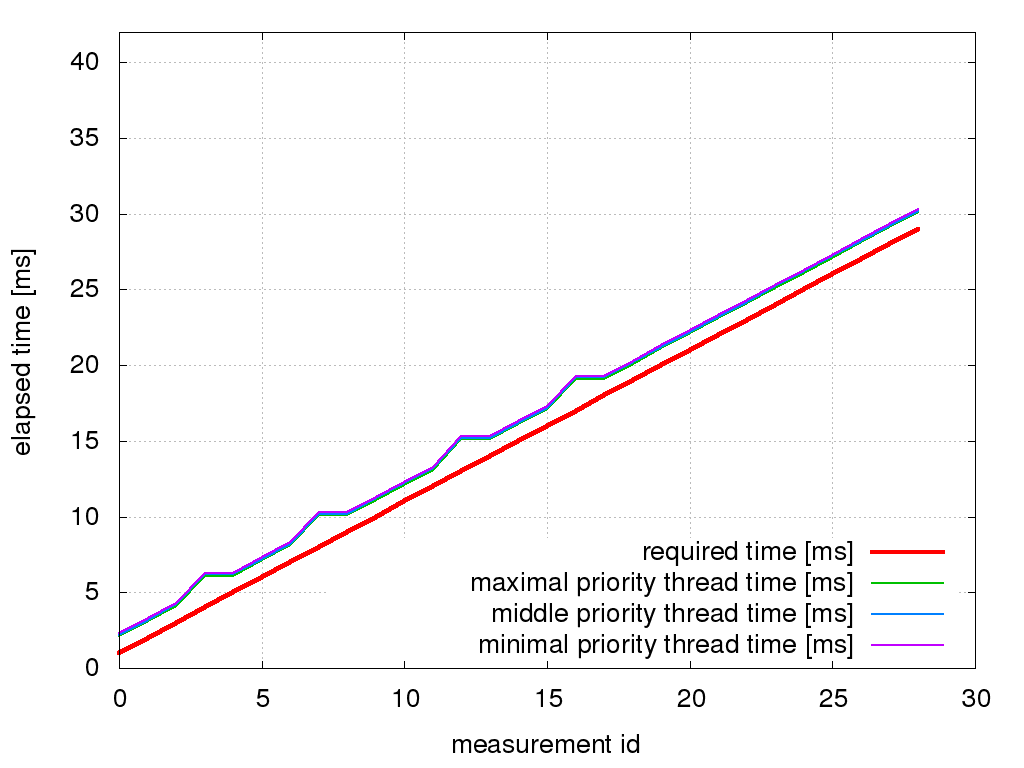
\includegraphics[width=3.4in]{round_robin_scheduler_perfomance.png}
\caption{Round robin real-time test}
\label{fig_round_robin_scheduler_perfomance}
\end{figure}


\begin{figure}[]
\centering
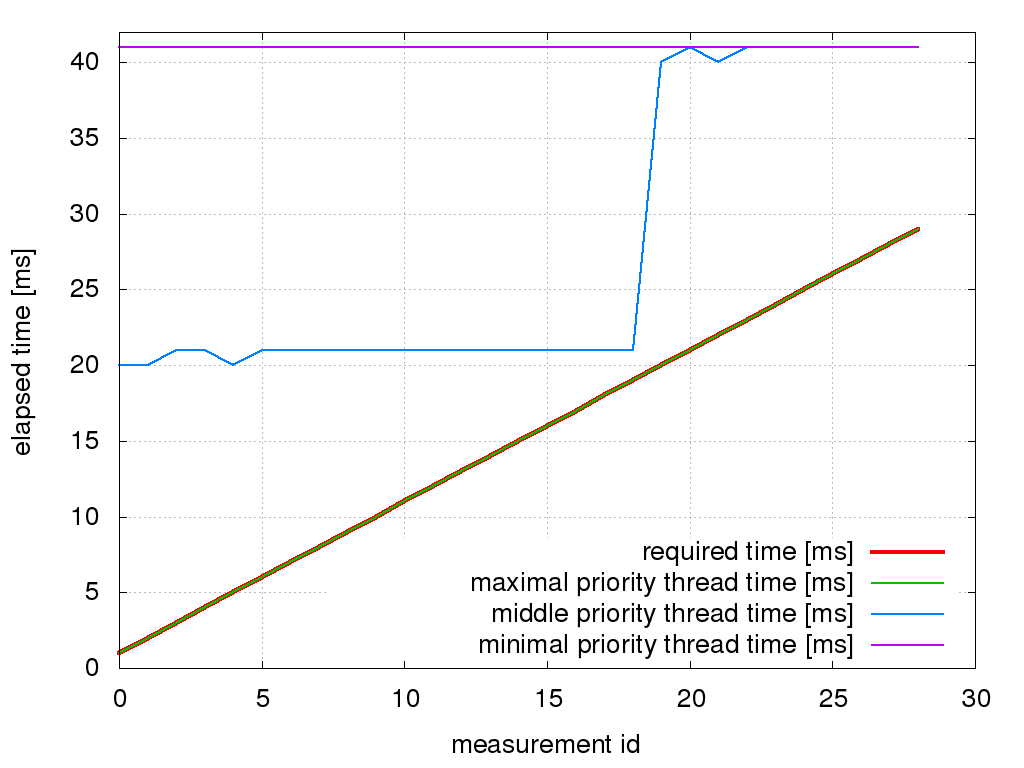
\includegraphics[width=3.4in]{priority_scheduler_perfomance.png}
\caption{Priority scheduler real-time test}
\label{fig_priority_scheduler_perfomance}
\end{figure}



Next testing was focused on the real-time processing ability. There were two main and six child threads (only first three are shown in figures). Each thread was waiting specified time (required waiting time) and this time was measured. Difference between required and measured time was used to compare round robin and priority scheduler scheduling algorithms.
\balance
We can see round robin results in the Fig. \ref{fig_round_robin_scheduler_perfomance} (all threads have same results). It can be seen, that required value is bellow measured lines and the time difference is around 1ms. Little peaks are consequence of timer resolution, which is 1ms.
Situation with priority scheduler can be seen in the Fig. \ref{fig_priority_scheduler_perfomance}.




Threads with the maximum priority perfectly meet the conditions. Threads with lower priorities were executing for much longer time. Following priority values $p_i$ have been used:

\begin{itemize}
	\item PRIORITY\_MAX = 8
	\item PRIORITY\_MID = 128
	\item PRIORITY\_MIN = 255
\end{itemize}


\begin{figure}[h]
\centering
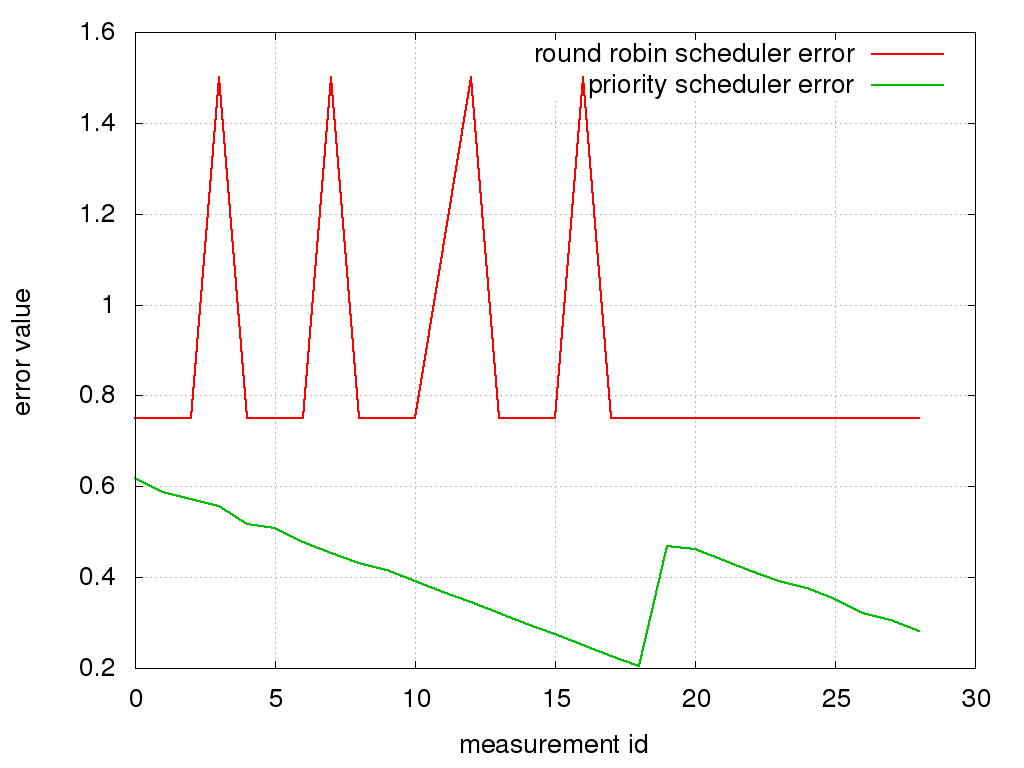
\includegraphics[width=3.4in]{scheduler_error.png}
\caption{Schedulers error comparison}
\label{fig_error}
\end{figure}

\begin{figure}[H]
\centering
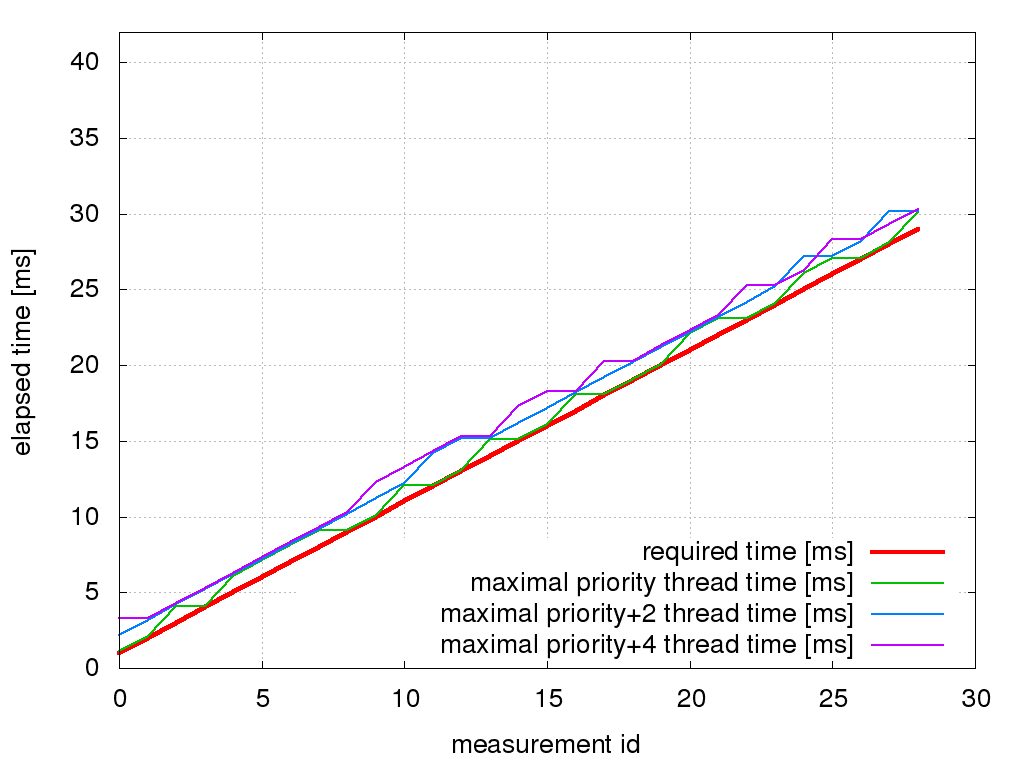
\includegraphics[width=3.4in]{priority_scheduler_similar_priority.png}
\caption{Priority scheduler real-time test with similar priorities}
\label{fig_priority_scheduler_similar_priority}
\end{figure}


We can use (\ref{error_eq}) to compute total error from meassured times. Result is shown in the Fig. \ref{fig_error}. From priority scheduling algorithm, it can be seen that it converges into round robin when priorities are equal. This experiment was accomplished and results are presented in the Fig. \ref{fig_priority_scheduler_similar_priority}.



\section{Conclusion}
In this paper, priority scheduler has been explained and OS was briefly introduced. From experimental results, we can see that priority scheduler has better results, when considering error function definition (\ref{error_eq}). Of course, if we consider maximal deadline time without looking for priorities, round robin has better results. For applications, where same priority is necessary, round robin (or priority scheduler with same priorities represented in the Fig. \ref{fig_priority_scheduler_similar_priority}) provides better solution. For applications, where it is needed to prioritize some processes, priority scheduler is of course better choice.



% serves to balance the column lengths on the last page of the document
% should be inserted the left column of the last page
\balance

 \bibliographystyle{plain}
\begin{thebibliography}{99}

\bibitem{bib:rad} Whill Hentzen, The Software Developer's Guide, 3rd Edition, ISBN: 1-930919-00-X, 2002


\bibitem{bib:wsn_applications1} John A. Stankovic, Anthony D. Wood, Tian He, Realistic Applications for Wireless Sensor Networks, http://www.ent.mrt.ac.lk/dialog/documents/ERU-2-wsn.ppt

\bibitem{bib:wsn_applications2} Nuwan Gajaweera, Wireless Sensor Networks, http://www.ent.mrt.ac.lk/dialog/documents/ERU-2-wsn.ppt

\bibitem{bib:lm4flash} LM4 flahsing tool, https://github.com/utzig/lm4tools/tree/master/lm4flash

\bibitem{bib:ti_launchpad} Texas instruments TivaC Launchpad, http://www.ti.com/tool/ek-tm4c123gxl

\bibitem{bib:suzuha_git}
Suzuha OS sources https://github.com/michalnand/suzuha\_os

\bibitem{bib:round_robin} Ishwari Singh Rajput and Deepa Gupta : A Priority based Round Robin CPU Scheduling Algorithm for Real Time Systems, ISSN: 2319 1058, 2012


\end{thebibliography}




\end{document}
